\section{A Method Concerning Propitious and Impropitious Times with Reference to One-Half, One-Third, and Two-Thirds of the Rising Times and the Periods of the Stars (5K,6P)}

We have set out here the systems which we have discovered with long, persevering investigation and which we have confirmed from our study of nativities. Now we append the topic of propitious and
impropitious times, about which the King and Petosiris spoke in riddles. Even if this system seems to our readers to be complicated and entangled, these readers may still marvel at the quality of its predictive force and its scientific effectiveness. 

The \mn{prediction} procedure of finding one chronocrator among the stars (the procedure characteristic of the other methods) and from this one to predict the future, <and to say> that the same star receiving the chronocratorship in the cycle of time will forecast the same matters, seems to me to be ignorance and error. For one star, according to its own nature, will bring about good or bad in the year <in question>, or in two or three years. 

We find in one period of time, either months or days, differing results occurring, mixtures of bad and good—we gain confidence that these are the facts, because in a given nativity we find at one time rank, stewardships, accusations, exile; or at another time a distinguished office, grievous pain, and weakness; or similarly a governorship, the possession of a livelihood, and death. We find some men unfortunate in their health, but lucky in their livelihoods, some \textbf{/278K/} troubled in their wives and their occupations, but strong and cheerful. So we do not think that these things come from one chronocrator, but from many. And the good that had been indicated is dissipated by the power of malefics, likewise the bad by the power of benefics.

Wherefore the Compiler says some things are unavoidable, other things are not. \hl{Unavoidable things occur when malefics happen to be activating something by themselves; avoidable things, when a benefic is involved while the malefics are operating \textbf{/266P/} and breaks up their power}. 

\hl{When a configuration of a benefic is found in a nativity and that benefic is found to be the chronocrator, the good results will be total,
but (as before) if the chronocratorship of malefic aspects is also operative, both good and bad will occur}—\hl{according to the nature of the stars and signs. In addition of course, the good and bad will come to pass proportionate to the greatness and the basis of the nativity}.

Just \mn{Basis} like the general forecasts for infant nativities: if we find that benefics are operative and are beholding the \Sun\, or the \Moon\, and the Ascendant from the right, we then promise length of life, rank, and the support of a livelihood. If malefics are operative, we consider the nativity to be unviable. It is necessary to examine the distribution of
chronocrators in the same way: in so far as benefics control, promise great success; if both are mixed, predict a similarly <mixed fortune>; if malefics alone enter into rule as chronocrators, predict dangers, ruin, and the onset of many crises.

So the King says:
\begin{quote}
“When the chronocratorships are plotted (i.e. those of the nativity) and when any are operative (he means any of the stars), if some other star comes into aspect or even has contact in the alternation of
chronocrators\footnote{Contact by ``handing off'' the times from one planet to another(?)}, the chronocratorship must be granted to both stars. For example, if the \Moon\, occupies the degree-position <of the chronocratorship> while some other star is also in the \Moon’s
sign, when the \Moon\, itself makes contact with the other place <=star>, it will control the chronocratorship of the sign, whether it is good or bad, or whether the associated stars are benefic or
the opposite. Moreover, if the star of \Jupiter\, happens to be in the aforementioned place, it will be indicative of rank, or of moderate rank plus the possession of a profitable livelihood. \textbf{/279K/} (He is
referring to the Lot of Fortune, the point indicative of possessions and benefits. The point concerning rank is a different one.) If a malefic is also in aspect or has contact with it, evil will come to pass in the chronocratorship of the benefics, as well as good. The time of the star which has attached itself is taken together and calculated with the other’s times. Whatever sum is arrived at, forecast that the results will occur toward the end of the periods and rising times. Now every star
which is at an angle gives its full period. (We have explained this in the preceding chapters.) \textbf{/267P/} The allotment of those which are not at the angles is subject to a deduction from their proper factors. (I think I have explained this matter in my book \textit{The Length of Life}.)

“In addition: suppose the \Moon\, controls the aforesaid place and the star of \Saturn\, is also there; the \Moon’s place (which is also the location of the star of \Saturn) is also in the Ascendant. Now the
complete period of \Saturn\, is 30 full years, that of the \Moon\, is 30 days\footnote{The minor period of \Saturn\, is 30 but the \Moon
s minor period is 25.}. Let the \Moon\, in its present sign be at an angle, let the star of \Mars\, either precede or follow the given sign so that it will make contact with it, and let the star of \Saturn\, have \Mars, the \Moon\, itself, or the \Sun\, in aspect. Men <with this horoscope> will be born of lowly parents. Add the chronocratorship of the sign in which the star of \Saturn\, is located and the chronocratorship of \Mars; this period will come into vicissitudes or will even cause travel. In the same chronocratorship, it will be the cause of injuries and wounds, particularly to the eyes. If the \Moon\, is waxing, but is not yet at the full moon, it indicates dimming of vision…and troubles happening to the eyes. \textbf{/280K/} Indeed it adds burns…and even cuts in the same places because \Mars\, is in contact with the Light-Bringer and hems it in with its burning heat.

“Next in order, forecast the effects of the star in aspect or in conjunction with the \Moon’s sign, if one or more happen to be located in the Lot <of Fortune>. Next forecast the stars following the
angles, in whatever Place they are located and whichever angle they follow.”
\end{quote}

We have cited this in his very words because of the following explanation. We have found it to be true by testing and long calculation.

Now if, as we have already said, the chronocratorship of one configuration takes effect at the time in question, when calculated from the total of the rising time of the sign and period of the star, then use the preceding rules. However, when combined chronocratorships are taking effect, attend to what is to be
predicted and determine the \textbf{/268P/} outcome using the positions of the angles and the stars preceding or following the angles, the positions of the Lots, and of the new and full moons, considering all of these according to the proper aspects or oppositions of the stars. 
If the chronocratorships of the aspects are combined, the results will come to pass in one-half, one-third, or two-thirds of the time, provided each one does not hold <the chronocratorship> alone.

It is necessary to investigate the contacts of the \Moon: if its configuration with another star is not in the same sign, but is in the next sign, then add the times of both stars (or the rising times of the signs in which they are located) and make the prediction. 

The consideration of the chronocrators is quite complex, sometimes involving the \Moon’s path and the Lot, sometimes the angles, sometimes the eastern, western, and other (i.e. when the stars are at a standstill) phases. The chronocrators must be understood as the
results of the interaction of malefics and benefics.

…As for my statement about one-half, one-third, or two-thirds of the time: the cut will come at the Place of Injuries if you calculate the distance in degrees. We have also discovered this in our discussion of
propitious and impropitious times… a fragment .

\begin{wrapfigure}[14]{R}{7cm}
\centering
\vspace{-10pt}
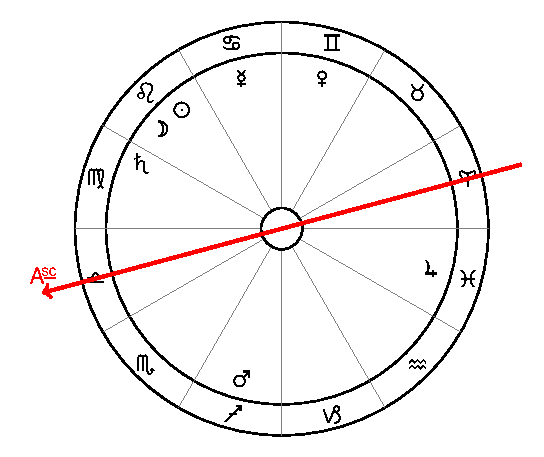
\includegraphics[width=.68\textwidth]{charts/7_6_01}
\caption{Chart 82 [VII.6.1, GH L124]}
\label{fig:chart82}
\end{wrapfigure} 

For example: \Sun, \Moon\, in \Leo, \Saturn\, in \Virgo, \Jupiter\, in \Pisces, \Mars\, in \Sagittarius, \Venus\, in \Gemini, \textbf{/281K/} \Mercury\, in \Cancer, Ascendant in \Libra, klima 7\footnote{\textit{Greek Horoscopes} dates the chart to July 29, 124 CE at about 10 a.m.}. 

In his 37th year he suffered a lawsuit about an inheritance on account of his wife, from whom he had expected great benefits. He lost the case at the king’s court. This time was not altogether injurious except insofar as it disappointed his hopes. The \Moon\, trine with \Mars\, indicated the 37th year: 25 for the \Moon\, plus 12 for \Sagittarius\, <=\Jupiter> total 37. Likewise \Jupiter\, and \Mercury\, <trine>: 12 for \Jupiter\, plus 25 for \Cancer\, <=\Moon> total 37\footnote{From minor periods of the \Moon\, (25) and \Jupiter\, (12).}. 

Investigating in the way we have explained, we find the opposition of \Mars\, and \Venus\, to be similarly operative in klima
7, as is \Saturn, which is square <with both>: 27 for \Gemini, 8 for \Venus, plus 20 for \Virgo <=\Mercury> total 55, two--thirds of which is 36 years, 8 months\footnote{The rising time of \Gemini\, in klima 7 of System A for Alexandria is 27°. \Virgo\, is alloted 20, the minor period of its ruler, \Mercury, and \Venus\, is allotted 8 for her minor period.}. \Pisces\, <=\Saturn>\footnote{\Saturn\, should probably read \Jupiter. The rising times of \Pisces\, in klima 7, System A for Alexandria are 15°, \Jupiter\, in and ruling \Pisces\, gives 12 for his minor period and \Saturn\, in opposition gives 30 for his minor period which adds to 57, 2/3 of which is 38, not far off 37 or 36 years, 8 months.} also indicated the same amount, but the malefics were strong\footnote{Schmidt, following Pingree, amends ``malefics'' to ``benefics'', linking it to the next sentence which says \Venus\, rules the Lot (VRS7 p.51); however, \Saturn\, is afflicting \Mars\, by a superior square and \Mars, who is contrary to the chart sect, is afflicting \Jupiter\, by superior square and \Venus\, by opposition while \Jupiter\, is being opposed by \Saturn.}. 

\Venus\, was the ruler of the Lot of Fortune <\Libra>. The native had won the same lawsuit in his 35th year, but when it was appealed, he lost. The 35 had good luck because of the rising time of \Pisces, 15, and \textbf{/269P/} of \Gemini\, <=\Mercury>, 20, plus \Gemini\, again, 27 <its rising time> and \Venus, 8, for a total of 35. Or 20 for \Gemini, and 15 for \Mars\, total of 35. Or 20 for \Virgo\, <=\Mercury> plus 15 for \Mars\, total 35. So both benefics and malefics were operative\footnote{Here \Venus\, and \Mars's are active, and there is some influence from \Jupiter\, via \Pisces, but \Saturn\, is not active as he is in the native's 37th year when the native loses his appeal.}, and since they were in bicorporeal signs, it will be necessary <to use> them several times <in making the forecast>\footnote{Bicorporeal (mutable) signs are an indication events will involve starts and stops and drag out over a period of time; events change or mutate. Fixed signs indicate a steady state of affairs or a recurring situation. Cardinal signs indicate a new event with each activation.}. 

Now \mndl the fact that malefics are in superior aspect and in opposition has great power. Wherefore Petosiris himself said, “The chronocratorships must be understood as the results of the interaction of benefics and malefics.” 

\newpage
\begin{wrapfigure}[14]{R}{7cm}
\centering
\vspace{0pt}
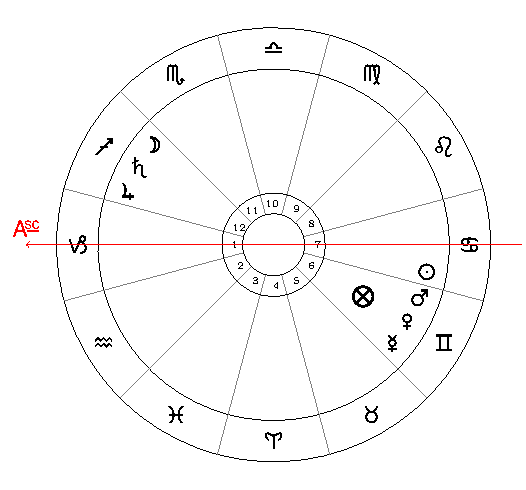
\includegraphics[width=.68\textwidth]{charts/7_6_02}
\caption{Chart 83 [VII.6.2, GH L134, VI]}
\label{fig:chart83}
\end{wrapfigure} 

The horoscope of the wife who lost the lawsuit is as follows: \Sun\, in \Cancer, \Moon, \Saturn, \Jupiter\, in
\Sagittarius, \Mars, \Venus, \Mercury\, in \Gemini, Ascendant in \Capricorn, klima 7\footnote{\textit{Greek Horoscopes} dates the chart to June 23, 134 CE about sunset}.

In her 25th year she seemed destined to win her case\footnote{According the text of the previous chart, she lost her case and her husband won.}, for the \Moon\, being with \Jupiter\, and \Saturn\, indicated 25, and the \Sun\, in \Cancer <=\Moon> also signified 25. In addition, the rest of the stars were operative by combination and opposition: 30 years for \Saturn\, plus 20 for \Mercury\, in opposition total 50, one-half of which is 25. Or 30
years for \Saturn\, plus 20 for \Mercury\, plus 25 for the \Moon\, total 75, one-third of which is 25. From that time the affair reversed itself: when the appeal was made in her 27th year, she was defeated\footnote{According to the text of the previous chart, she won her appeal in this year and her husband's earlier win was reversed.}. 

The rising time of \Gemini\, <27>\footnote{The rising time for \Gemini\, in klima 7 of System A for Alexandria.} was operative, the location of the Lot of Fortune accompanied by \Mars\, and \Mercury. Additionally, 25 for the \Moon\, \textbf{/282K/} plus 15 for \Mars\, in opposition total 40, two-thirds of which is 26 years, 8 months. Here too the stars happened to be in bicorporeal signs.

\newpage
\begin{wrapfigure}[14]{R}{7cm}
\centering
\vspace{0pt}
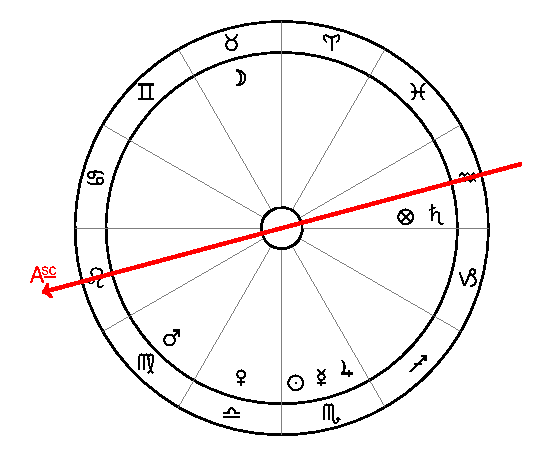
\includegraphics[width=.68\textwidth]{charts/7_6_03}
\caption{Chart 84 [VII.6.3, GH L108, XI]}
\label{fig:chart84}
\end{wrapfigure} 

Another example: \Sun, \Mercury, \Jupiter\, in \Scorpio, \Moon\, in \Taurus, \Saturn\, in \Aquarius, \Mars\, in \Virgo, \Venus\, in \Libra, Ascendant in \Leo, klima 2\footnote{\textit{Greek Horoscopes} dates the chart to November 6, 108 CE about midnight}.

In his 52nd year he had a very great quarrel and a lawsuit with his sister about property and an inheritance, and he won at the king’s court. 

The configuration of opposition was operative: 25 for the \Moon, 12 for \Jupiter, 15 for \Scorpio\, <=\Mars>, for a
total of 52. Additionally in klima 2, 36 for \Scorpio\footnote{The rising time for \Scorpio\, in klima 2, System A for Alexandria is 35°40'.}, 12 for \Jupiter, 30 for \Saturn\, (in the sign of the Lot of Fortune) total 78, two-thirds of which is 52. Or again, 24 for \Taurus, 24 for \Aquarius\footnote{The rising times for \Taurus\, and \Aquarius\, (who rise together) in klima 2, System A for Alexandria, are 24°20'.}, plus 30 for \Saturn total 78, two-thirds of which is 52. 

So all the stars except \Mars\, were operative. He was ill at that time, had a narrow escape at sea, and made great expenditures, but the benefics seemed to be in superior aspect to \Saturn\, and were more powerful.

\newpage 
\begin{wrapfigure}[15]{R}{7cm}
\centering
\vspace{0pt}
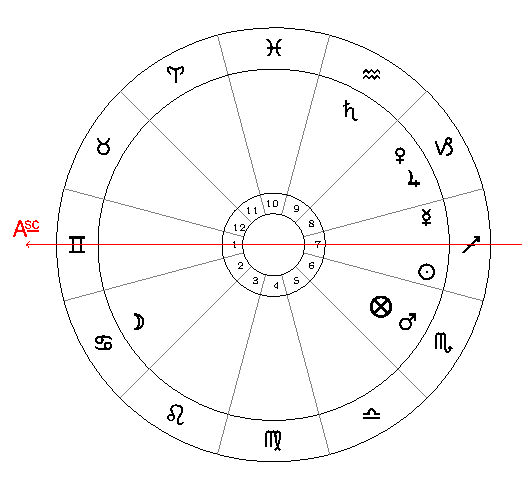
\includegraphics[width=.68\textwidth]{charts/7_6_04}
\caption{Chart 85 [VII.6.4, GH L110, XII]}
\label{fig:chart85}
\end{wrapfigure} 

\noindent\textbf{/270P/} The horoscope of the sister who lost the lawsuit is as follows: \Sun, \Mercury\, in \Sagittarius, \Moon\, in \Cancer, \Saturn\, in \Aquarius, \Jupiter, \Venus\, in \Capricorn, \Mars\, in \Scorpio, Ascendant in \Gemini, klima 4\footnote{\textit{Greek Horoscopes} dates the chart to December 15, 110 CE about sunset. Schmidt gives ``klima 2'' and does not think the chart is related to the previous one as the events do not appear to happen around the same time (VRS7 p.56).}.

The 54th year is indicated by 30 for \Saturn\, plus 24 for \Venus, totalling 54. Or again 36 for \Scorpio\footnote{The rising time for \Scorpio\, in klima 4, System A for Alexandria is 37°00'; in klima 2, which Schmidt used, the rising time is 35°40'.}, plus 15 for \Mars, which was in the sign of the Lot of Fortune and which was operative, plus 30
for \Saturn\, total 81, two-thirds of which is 54. The dominant aspect of the malefics was operative. So in her 53rd year she had an apparent and supposed victory through the help of the great, and so she resorted to a lawsuit; this was because the \Moon\, allotted 25 and \Capricorn\, 28\footnote{The rising time for \Capricorn\, in System A for Alexandria, klima 4, is 27°40'; for klima 2, 28°06'40''.} for a total of 53. But in her 54th year
she was abandoned by her helpers, for the benefics did not combine to become chronocrators at that time.

\newpage
\begin{wrapfigure}[15]{R}{7cm}
\centering
\vspace{0pt}
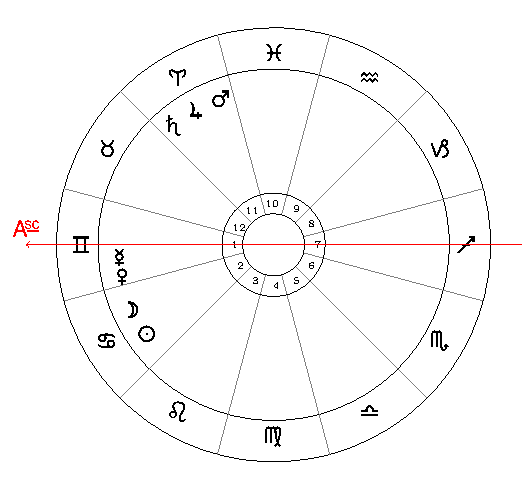
\includegraphics[width=.68\textwidth]{charts/5_10_13}
\caption{Chart 68a [VII.6.5, GH L113, VII]}
\label{fig:chart68a}
\end{wrapfigure} 

\noindent Another example: \Sun, \Moon, in \Cancer, \Saturn, \Jupiter, \Mars\, in \Aries, \Venus, \Mercury, Ascendant in \Gemini, klima 1\footnote{This is the same chart given in Book 5 Section 13.}

In his 47th, 48th, and 49th years he was ill, suffered a great flow of blood, and was enfeebled. At the same time he was banished. 

The 47th year was indicated by 31;40 for \Cancer\footnote{The rising time for \Cancer\, in klima 1, System A for Alexandria is 31°40'.} plus 15 for
\Mars\, totalling 46 years, 8 months. The 48th year was indicated by 31;40 for \Cancer\, again, 25 for the \Moon, plus 15 for \Mars, for a total of 72, two-thirds of which is 48. Also in the 48th year the rising time of \Gemini, 28;20\footnote{The rising time for \Gemini\, in klima 1, System A for Alexandria is 28°20'.}, plus the period of \Mercury, 20, were operative, totalling 48 years, 4 months. At that time in his 49th year he found a little charity and support. The \Sun\, and \Saturn\, allotted 19 and 30 for a total of 49. The malefics in superior aspect to the \textbf{/283K/} luminaries were the cause of great dangers, and if \Jupiter\, had not been in the configuration, the malefics absolutely would have brought him violent death. 

\newpage
\begin{wrapfigure}[14]{R}{7cm}
\centering
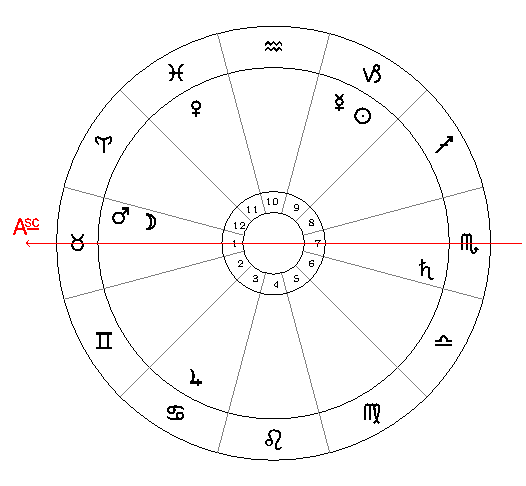
\includegraphics[width=.68\textwidth]{charts/7_6_06}
\caption{Chart 86 [VII.6.6, GH L129]}
\label{fig:chart86}
\end{wrapfigure} 

Another example: \Sun, \Mercury\, in \Capricorn, \Moon, \Mars, Ascendant in \Taurus, \Saturn\, in \Scorpio, \Jupiter\, in \Cancer, \Venus\, in \Pisces, klima 6\footnote{\textit{Greek Horoscopes} dates the chart to January 16, 129 CE about 2 p.m.}.

In his 30th year he escaped slavery, committed many robberies, avoided capture for a short time, but was caught in the same year. 

Both sets <of signs> in opposition were operative <\Taurus/\Scorpio, \Cancer/\Capricorn>: they both total 60, one-half of which is 30. Also 28 for \Capricorn\footnote{The rising time of \Capricorn\, in klima 6, System A for Alexandria is 27°13'20''.}, 20 for \Mercury, plus 12 for \Jupiter\, total 60, one-half of which is 30. Also 30 for \Saturn\, plus 15 for \Mars, two-thirds of which is 30. Also 25 for \Cancer\, <=\Moon>, 12 for \Jupiter, plus
8 for \Venus\, (which is trine) total 45, two-thirds of which is 30. 

Because of the benefics, he seemed destined to escape danger for a short time and \textbf{/271P/} to live comfortably from the takings of his robberies, but because of the malefics, he fell.

\newpage
\begin{wrapfigure}[15]{R}{7cm}
\centering
\vspace{0pt}
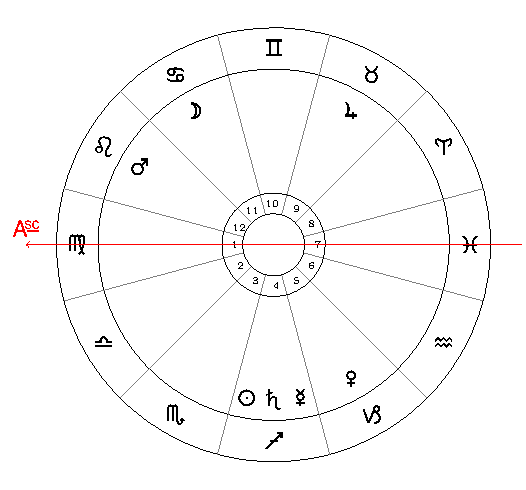
\includegraphics[width=.68\textwidth]{charts/7_6_07}
\caption{Chart 87 [VII.6.7, GH L102,XII,14] }
\label{fig:chart87}
\end{wrapfigure} 

Another example: \Sun, \Saturn, \Mercury\, in \Sagittarius, \Moon\, in \Cancer, \Jupiter\, in \Taurus, \Mars\, in \Leo, \Venus\, in \Capricorn, Ascendant in \Virgo, klima 2\footnote{\textit{Greek Horoscopes} dates the chart to December 13, 102 CE about midnight}.

The native, although of governing rank, fell into the governor’s disfavor and was condemned to the mines/quarries in his 34th year. 
\Mars, together with the \Sun, controlled the chronocratorship: 19 for the \Sun\, plus 15 for \Mars\, total 34. In his 36th year, through the help of the great, he was released from confinement as disabled. 

At that time in his 36th year the rising time of \Leo\, was operative\footnote{The rising time of \Leo\, in klima 2, System A for Alexandria is 35°40''.}. In addition, 12 for \Jupiter\, in superior aspect <to \Scorpio, \Mars’s house> plus 24 for \Taurus\, also total 36. Also 28 for \Capricorn\footnote{The rising time for \Capricorn\, in klima 2, System A for Alexandria is 28°06'40''.}, plus 8 for \Venus\, total 36. So the benefics were powerful. 

In his 39th year trouble arose again because of the pre-existing hostility, and he was exiled to an island/oasis. The stars in \Sagittarius\, controlled this period: 19 for the \Sun, 20 for \Mercury\, for a total of 39. Also take two-thirds of 58, which is 38 years, 8 months. (19 for the \Sun, 20 for \Mercury, plus 19 for \Leo <=\Sun>, because \Mars\, is there in trine, total 58. Again for \Mars\, <in \Leo=\Sun> 19, plus 19 for the \Sun, plus 20 for \Mercury\, total 58.) 

In his 40th year he lived endangered and fell ill. His wife, however, accompanied him with affection, comforted him, and shared her property with him. 

The 40th year is indicated by the contact of the \Moon\, with \Mars\, (25 for the \Moon\, plus 15 for \Mars\, total 40), and the fact that \Jupiter\, and \Venus\, were trine showed the same, because \textbf{/284K/} 12 for \Jupiter\, plus 28 for \Venus\, <=\Capricorn> total 40. I myself had a hand in these forecasts.

\newpage
Another example: \Sun, \Mercury\, in \Capricorn, \Moon, \Saturn\, in \Sagittarius, \Jupiter\, in \Cancer, \Mars\, in \Virgo, \Venus\, in \Aquarius, Ascendant in \Libra, klima 2\footnote{This chart was first given in Book II, Section 2.}

\begin{wrapfigure}[15]{R}{7cm}
\centering
\vspace{0pt}
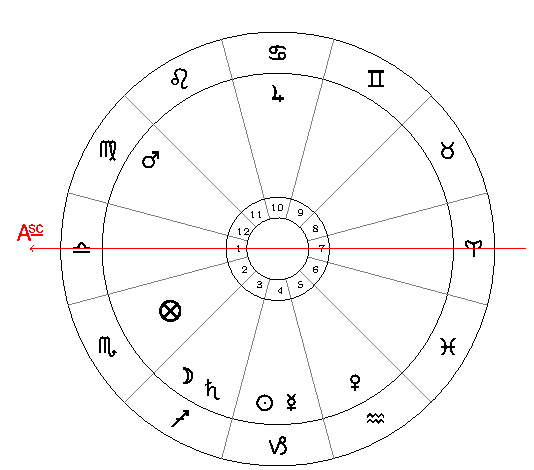
\includegraphics[width=.68\textwidth]{charts/7_6_08}
\caption{Chart 11a [VII.6.8, GH L105] }
\label{fig:chart11a}
\end{wrapfigure} 

In his 48th year he saw the death of his beloved son, a very great sorrow, and in the same year the death of his mother. \Virgo\, and \Libra\, indicated this because of their equal rising times <40>\footnote{The rising time for both \Virgo\, and \Libra\, in klima 2, System A for Alexandria is 37°26'40'' but for Babylon it is 40°00'.}: 8 years for \Libra\, <=\Venus> plus 40 for \Virgo\, total 48. Since \Mars\, was found with the Ascendant, it brought grief with respect to the mental/emotional factors\footnote{Schmidt states that, as \Mars\, is not in \Libra, but averse in \Virgo\, an equally rising sign, the aversion is mitigated and the mitigation is equivalent to \textsl{co-presence} i.e. being in the same sign (VRS7 p63). It is also possible that \Mars\, can be considered ``with'' the Ascendant as \Mars\, is in a sign that is active (operative) at the same time as the Ascendant sign and so it participates in the rulership of the time.}. 

Additionally, 40 for \Virgo\, plus 32 for \Sagittarius\, total 72, two-thirds of which is 48.

\newpage

\begin{wrapfigure}[14]{R}{7cm}
\centering
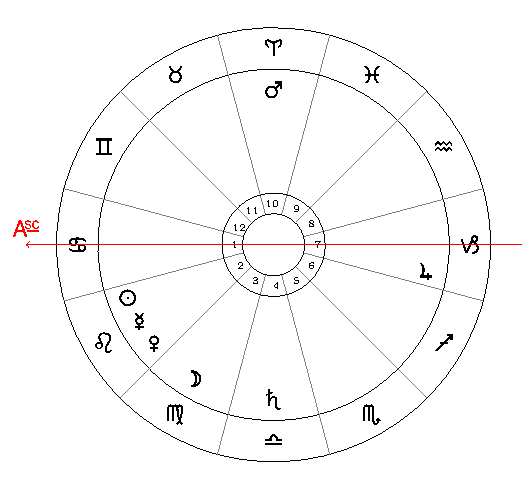
\includegraphics[width=.68\textwidth]{charts/7_6_09}
\caption{Chart 88 [VII.6.9, GH L158] }
\label{fig:chart88}
\end{wrapfigure} 

Another example: \Sun, \Mercury, \Venus\, in \Leo, \Moon\, in \Virgo, \Saturn\, \textbf{/272P/} in \Libra, \Jupiter\, in \Capricorn, \Mars\, in \Aries, Ascendant in \Cancer, klima 6\footnote{\textit{Greek Horoscopes} dates the chart to August 14, 158 CE about 4 a.m.}.

From observation I made note of these chronocratorships, and since the nativity was that of an infant, \mndl I calculated them as months, not years. At the completion of his eighth month and for part of his ninth, he was subject to convulsions and was almost in danger of dying. The eighth month was indicated by \Libra\, <=\Venus>, with \Saturn\, in that sign. Half of the ninth month was indicated by the rising time of \Aries, 17\footnote{The rising time of \Aries\, in klima 6, System A for Alexandria is 16°06'40''.}, operative until the completion of 8 months, 15 days. Additionally, the rising time of \Capricorn\, was operative to the same effect: one-third of its rising time, 27\footnote{The rising time of \Capricorn\, in klima 6 of System A for Alexandria is 27°13'20''.}, is 9; 19 for the \Sun\, plus 8 for \Venus\, total 27, one-third of which is 9. 

There were indications in the other months which were controlled by malefics: he suffered from boils and eczema in (for example) the 15th, the 17th, the 27th and other months, particularly the 27th. The cause was this: when playing with
an animal he fell and was injured in the generative organs. The 27th month was indicated by \Mars\, and the \Moon: 15 for \Mars\, plus 25 for the \Moon\, total 40, two-thirds of which is 26 months, 20 days. (I consider \Aries\, and \Virgo\, to be in opposition because <the \Moon> was moving toward it <opposition>\footnote{Schmidt believes this is a joining by sign as, according to Neugebauer's calculations the \Moon\, is 23 degrees from an opposition to \Mars. He also believes the opposition is considered operative as the two signs, \Virgo\, and \Libra\, have equal rising times which would mean they'd become active at the same time (VRS7 p.65). This is similar to Valens statement about chart VII.6.8 where he assigned ``co-presence''  when \Mars\,s and the Ascendant were in signs with equal rising times.}.) 

Additionally, 15 for \Mars\, plus 25 for the Ascendant in \Cancer\, <=\Moon> total 40, two-thirds of which is 26 months 20 days. But in that month the rising time of \Capricorn, 27, was also operative; 15 for \Mars\, plus 12 for \Jupiter\, total 27; or again 19 for the \Sun\, plus 8 for \Venus\, total 27. 

From this 28th month he lived precariously: the rising time of \Libra\, and the period of \Saturn\, coincided. 

In his 32nd month he was dangerously ill and was in convulsions: 15 for \Mars\, plus the rising time of \Aries, 17 total 32. 

In his 33rd month he died: the rising time of \Cancer\, equalled this figure. \textbf{/285K/} Additionally 25 for \Cancer\, <=\Moon> plus 8 for \Libra\, <=\Venus> total 33, as does 25 for the \Moon\, plus 8 for \Libra. I calculated as if the \Moon\, were in \Libra\, with \Saturn, which is permissible because of the equal rising times <of \Virgo\, and \Libra>.

\newpage
Another example: \Sun, \Mercury\, in \Libra, \Moon\, in \Aquarius, \Saturn\, in \Pisces, \Jupiter\, in \Capricorn,
\Mars\, in \Aries, \Venus\, in \Leo, Ascendant in \Cancer, klima 6\footnote{\textit{Greek Horoscopes} dates the chart to September 30, 111 CE about midnight}.

\begin{wrapfigure}[15]{R}{7cm}
\centering
\vspace{0pt}
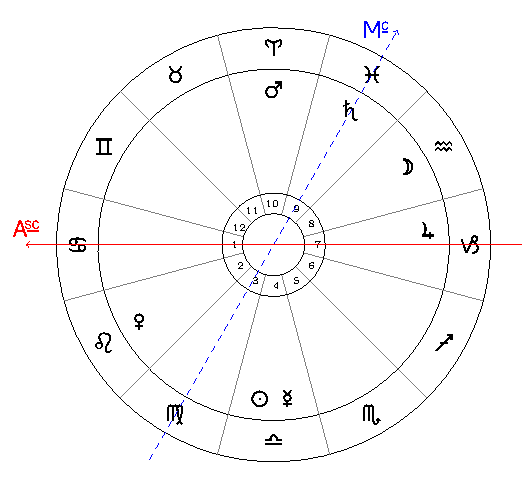
\includegraphics[width=.68\textwidth]{charts/7_6_10}
\caption{Chart 89 [VII.6.10, GH L111, IX] }
\label{fig:chart89}
\end{wrapfigure} 

The native was rich, but in his 47th year he was exiled, for \Saturn\, was operative at MC, the IX Place, as was the rising time of \Pisces: 30 for \Saturn\, plus 17 for \Pisces\footnote{The rising time for \Pisces\, in klima 6, System A for Alexandria is 16°06'40''.}, total 47. 

In addition the fact that the \Sun\, and \Mercury\, were in opposition to \Mars\, <was operative>: 15 for \Mars, 17 for the rising time of \Aries\footnote{\Aries\, has the same rising time as \Pisces.}, 19 for the \Sun, plus 20 for \Mercury\,\footnote{and 38 for \Leo - marginal note [Riley]. \Leo\, has a rising time in klima 6, System A for Alexandria of 38°20'.} total 71, two-thirds of which is 47 years, 4 months. In addition the square configuration of \Libra\, and \Capricorn\, <was operative>: 27 for \Capricorn\, plus 20 for \Libra\, total 47\footnote{\Capricorn\, has a rising time of 27°13'20'' and \Libra\, has one of 43°53'20'' in klima 6, System A for Alexandria which does not add to 47. Schimdt says ``20 of \Mercury'' (VRS7 p.68) which is in \Libra, 27 and 20 does give 47.}. To all appearances, he seemed to be protected all around, but he endured reverses and losses because of a woman.

It \mndl is absolutely necessary to prove the appended topics: \Saturn\, at MC for night births is indicative of exile <as in the previous nativity>. \Mars\, following MC for day births forecasts the same. 

If the ruler of MC is in aspect to the right with MC or is operative, then after the exile, there will be recovery and restoration beginning with the chronocratorship indicated by the rising time of the sign or by the cyclical return of the star. 

The \Sun\, operative at night at IC without a houseruler, or the \Moon\, at MC, forecasts a precarious nativity. 

New or quarter moons with \Saturn\, in square, opposition, or conjunction are indicative of exile. Likewise full or first quarter moons with \Mars\, in opposition, square, or conjunction indicate great ruins and disaster, dooms that are far-famed in song and story. If they are in solid signs and degrees, the native is laid low once and for all; if they are in bicorporeal signs, often; if in tropic signs, they defame men far and wide; if they are at the angles, the native goes from the greatest good fortune to the greatest bad fortune; if they follow the angles, they make the native suffer and expect changes, one after the other; if they precede the angles, they involve him in downfall, kidnapping or banditry, violence, tortures, \textbf{/286K/} and a miserable death. 

It is hard on a night birth to have the \Moon\, (for a day birth, the Sun) precede an angle. If the malefics are square with the \Sun\, and \Moon, the native is dragged into large-scale warfare and uprisings, and he is killed.

In \mndl general, \Saturn\, opposed to \Mars\, is not good for either a free man or a slave: ill fortune will extend far. When in square or opposition, these stars make toilsome and troubled men. 

It is best if such configurations of these stars precede the angles, because if they occur at the angles, they bring death to <good> fortune and danger to occupations and to the whole basis <of the nativity>. 

If they follow the angles, they cause expected good to turn to the worse, they repress enterprises, \textbf{/274P/} and they make fortunes toilsome and wearisome. 

If they precede the angles, there are complex but understandable changes regarding livelihood for those who are endowed with such a configuration. If, however, benefics are in aspect with the above-mentioned configuration, the bad will be less or can be alleviated.

The \mnt same effects occur when they rule the configurations in the distribution of the chronocratorships. Since most stars—indeed all—seem to be chronocrators, the determination of good or bad results will be made from the transits at any given time, particularly when the chronocrator transits operative places and has some connection with the affairs of the nativity. Then it shows results which can be securely
forecasted.

\begin{wrapfigure}[15]{R}{7cm}
\centering
\vspace{-2em}
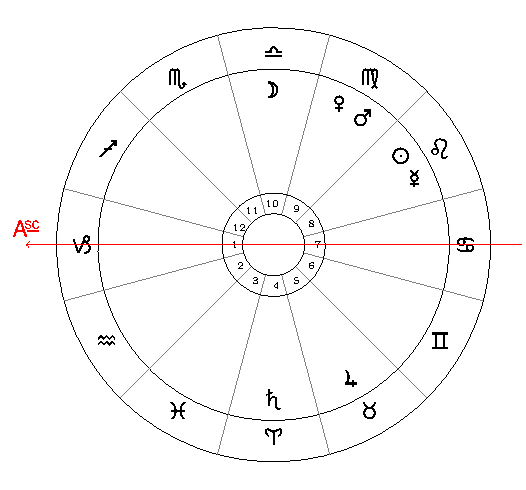
\includegraphics[width=.68\textwidth]{charts/7_6_11}
\caption{Chart 90 [VII.6.11, GH L114, VII] }
\label{fig:chart90}
\end{wrapfigure} 

<To show> that nature is astonishing and that nothing happens apart from the will of Fate—yea, even those lost in wars, collapses, fires, shipwrecks, or any other disaster are altogether governed by Fate—I will append a short illustrative example\footnote{The next six example charts are all of men who were involved in a shipwreck.}: \Sun, \Mercury\, in \Leo, \Moon\, in \Libra, \Saturn\, in \Aries, \Jupiter\, in \Taurus, \Mars, \Venus\, in \Virgo, Ascendant in \Capricorn, klima 2. 

In his 40th year he had a critical point: 25 for the \Moon\, plus 15 for \Aries\, <=\Mars> total 40, or 20 for \Aries, (in opposition <to the \Moon>) plus 40 for \Libra\footnote{The rising time for \Aries\, in klima 2, System A for Alexandria is 20°33'20''; in System A for Babylon, 20°00'. For \Libra\, they are 37°25'40'' and 40°00'.}, total 60, two-thirds of which is 40. The point was critical by a multiple of two: at the same time I found 28 for \Capricorn, the Ascendant\footnote{The rising time for \Capricorn\, in klima 2, System A, for Alexandria, is 28°06'40'' and for Babylon 28°00''.}, plus 12 for \Jupiter\, trine, for a total of 40; or again 30 for \Capricorn\, <=\Saturn>, 22 for \Taurus\footnote{The rising time for \Taurus, in klima 2, System A for Alexandria is 24°20' and for Babylon, 24°00. It's not clear where Valens got the 22 from.}, plus <\Venus’s> period, 8, for a total of 60, two-thirds of which is 40.

\newpage
\textbf{/287K/} Another example: \Sun, \Mercury\, in \Aquarius, \Moon\, in \Scorpio, \Saturn\, in \Cancer, \Jupiter\, in \Libra, \Venus\, in \Capricorn, \Mars, Ascendant in \Virgo, klima 7\footnote{\textit{[This chart was first introduced in Book V, Section 9]}}.

\begin{wrapfigure}[15]{R}{7cm}
\centering
\vspace{-20pt}
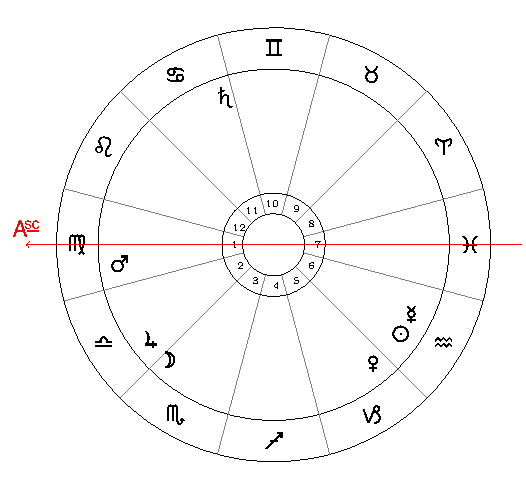
\includegraphics[width=.68\textwidth]{charts/5_09_1}
\caption{Chart 54a [VII.6.12, GH L120, II] }
\label{fig:chart54a}
\end{wrapfigure} 

In his 35th year he had a criticial point: \Mars’ period, 15 years, and \Virgo’s <=\Mercury’s>, 20, were operative for a total of 35. In addition 8 for \Venus\, plus 27, the rising time of \Capricorn, total 35. Or again 30 for \Saturn, in opposition <to \Venus>
plus 32;30 for \Cancer\, plus 8 for \Venus\, total 70 years 6 months, one-half of which is 35 years, 3 months. Additionally \Jupiter\, and \Saturn\, shared the chronocratorship, because 42 years 6 months for \Libra\, plus 27 years, 6 months for \Cancer\, totalled 70 years, one-half of which is 35.

\newpage
\begin{wrapfigure}[15]{r}{7cm}
\centering
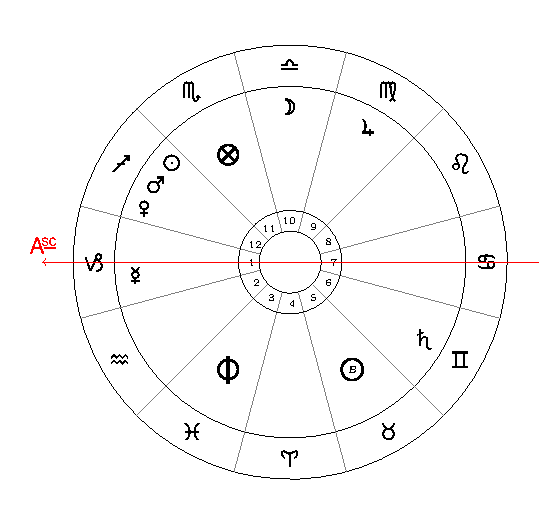
\includegraphics[width=.68\textwidth]{charts/7_6_13}
\caption{Chart 21b [VII.6.13, GH L118] }
\label{fig:chart21b}
\end{wrapfigure} 

Another example: \Sun, \Mars, \Venus\, in \Sagittarius, \Moon\, in \Libra, \Saturn\, in \Gemini, \Jupiter\, in \Virgo, Ascendant, \Mercury\, in \Capricorn \footnote{This chart was introduced in Book II, Section 2 and used again in Book V, Section 3.  Greek Horoscopes says there is a typo here and \Mercury\, is really in \Scorpio}, klima 6. 

At age 36 1/2 he had a critical point: 27 years 6 months\footnote{This is most likely for \Gemini (GH. p.115) which has rising times of 27°13'20'' in System A for Alexandria.}, plus 8 for \Venus, total 35 years \textbf{/275P/} 6 months. Add 19 for the \Sun\, (for \Gemini)\footnote{\Sun\, is in \Sagittarius, based on GH text is likely ``\Sun\, 19 years and 35 years 6 months for \Sagittarius.'' (p.115)}, and the total is now 54 years 6 months, two-thirds of which is 36 years 4 months. The benefics also had a share in these matters. 

\newpage
\begin{wrapfigure}[15]{r}{7cm}
\centering
\vspace{0pt}
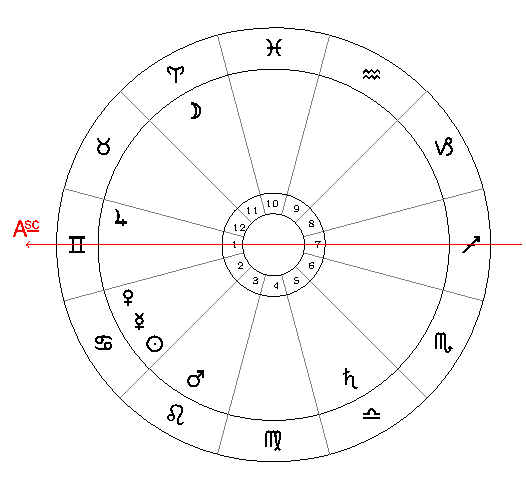
\includegraphics[width=.68\textwidth]{charts/7_6_14}
\caption{Chart 91 [VII.6.14, GH L127,VII] }
\label{fig:chart91}
\end{wrapfigure} 

Another example: \Sun, \Mercury, \Venus\, in \Cancer, \Moon\, in \Aries, \Jupiter, Ascendant in \Gemini, \Saturn\, in \Libra, \Mars\, in \Leo, klima 1\footnote{\textit{Greek Horoscopes} dates the chart to July 18, 127 CE about 4 a.m.},

In his 27th year he had a critical point: 19 for the \Sun\, plus 8 for \Libra\, <=\Venus> total 27. 

Additionally 28 years, 4 months for \Gemini\footnote{The rising times for \Gemini\, in klima 1, System A for Alexandria are 28°20'00''.}, plus 12 for \Jupiter\, total 40 years 4 months, two-thirds of which is approximately 27. Again 19 for \Leo\, <=\Sun>, 31 years, 8 months for \Cancer\footnote{The rising times for \Cancer\, in klima 1, System A for Alexandria are 31°40'00''.}, plus 30 for \Saturn\, total 80 years, 8 months, one-third of which is approximately 27.

\newpage
\begin{wrapfigure}[15]{R}{7cm}
\centering
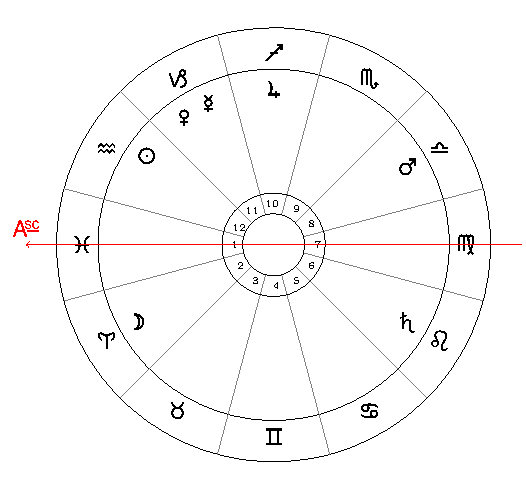
\includegraphics[width=.68\textwidth]{charts/7_6_15}
\caption{Chart 92 [VII.6.15, GH L122,I.30] }
\label{fig:chart92}
\end{wrapfigure} 

Another example: \Sun\, in \Aquarius, \Moon\, in \Aries, \Saturn\, in Leo, \Jupiter\, in \Sagittarius, \Mars\, in \Libra, \Venus, \Mercury\, in \Capricorn, Ascendant in \Pisces, klima 6\footnote{\textit{Greek Horoscopes} dates the chart to January 30, 122 CE about 8 a.m. and computes the value of \Venus\, as 22 \Aquarius}.

In his 33rd year he had a critical point: 25 for the \Moon\, plus 8 for \Libra\, <=\Venus> total 33. 30 for \Saturn\, and 19 for the \Sun\, total 49, two-thirds of which is 32 years, 8 months. 

In addition, the rising time of \Sagittarius\, <MC>, 33\footnote{The rising time for \Sagittarius\, in klima 6, System A for Alexandria is 32°46'40''.}, was operative, with \Jupiter\, in that sign.

\newpage
\begin{wrapfigure}[15]{R}{7cm}
\centering
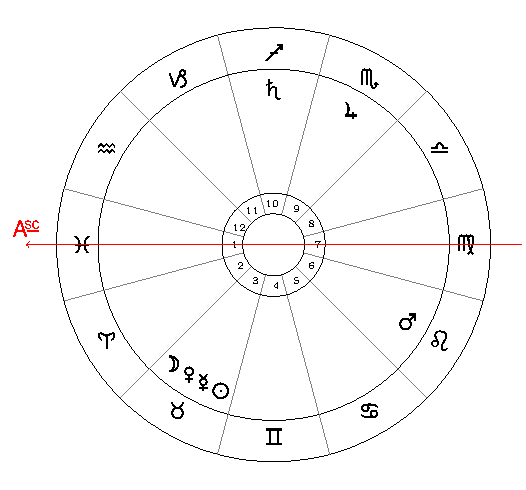
\includegraphics[width=.68\textwidth]{charts/7_6_16}
\caption{Chart 93 [VII.6.16, GH L133] }
\label{fig:chart93}
\end{wrapfigure} 

Another example: \Sun, \Mercury, \Venus, \Moon\, in \Taurus, \Saturn\, in \Sagittarius, \Jupiter\, in \Scorpio, \Mars\, in \Leo, Ascendant in \Pisces, klima 2\footnote{\textit{Greek Horoscopes} dates the chart to  April 24, 133 CE about 2 a.m.}.

In his 22nd year he had a critical point: 19 for \Leo\, <=\Sun> plus 25 for the \Moon\, total 44, one-half of which is 22. Additionally 36 for \Scorpio\footnote{The rising time for \Scorpio\, in klima 2, System A for Alexandria is 35°40'00''.}, plus 8 for \Taurus\, <=\Venus> total 44, one-half of which is 22.

These six men, while on a voyage with many others, encountered a violent storm and, with the rudder swept away, were in danger of drowning as the ship took on water. But \textbf{/288K/} because of the direction of the wind and the steersman’s management of the sails, they escaped. 

They encountered other dangers at that time, particularly a roving pirate ship. \mndl As a result, if—as often happens—many or all of the stars are found to be operative at the given period,
it is necessary to determine how each one is configured and which star’s aspect is the more opportune and powerful, the one causing good or the one causing bad; make that one the guidepost of your forecast. Then forecast according to the others which have a weaker effect, acting through hope, postponement, anxiety, and penalties.  Often even when the stars should show an obvious effect, they will be weak because another star prevails, being at a powerful place. If the influences derived from their configurations \textbf{/276P/} and signs are equal, then both bad and good will occur. 

Now often in regard to chronocratorships, unavoidable and vigorous angle-relationships <sextile trine square> are found to have a wide-ranging effect, and even when they seem to be leaving the chronocratorship, they again become powerful and <continue> ruling. As a result, even if another aspect is operative, it will not be vigorous since it is overcome by the previous aspect, particularly when a malefic is influential, being in opposition or in superior aspect.

Let us take an example: \Sun, \Saturn, \Mercury\, in \Aries, \Moon, \Jupiter\, in \Leo, \Mars\, in \Taurus, \Venus\, in \Aquarius, Ascendant in \Virgo, klima 1\footnote{\textit{Greek Horoscopes} dates the chart to March 25, 142 CE about 4 p.m.}.

\begin{wrapfigure}[15]{R}{7cm}
\centering
\vspace{-20pt}
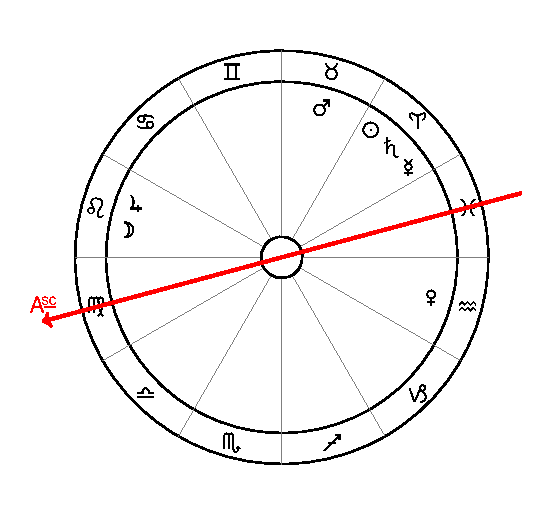
\includegraphics[width=.68\textwidth]{charts/7_6_17}
\caption{Chart 94 [VII.6.17, GH L142] }
\label{fig:chart94}
\end{wrapfigure} 

In his <16th> year he travelled abroad with a distinguished
woman because of her friendship and rank, and for further intimacy and erotic passion: \Aquarius\, <\Venus’s position> indicated 25 years\footnote{The rising time of \Aquarius\, in klima 1, System A for Alexandria is 25°00'00''.}, and if \Venus\, had been operative alone, it would have applied its benefic influence quickly. But as it was, \Mars\, controlled 25 years also, because of the rising time of \Taurus\footnote{\Taurus\, and \Aquarius\, are equally rising.}, and in addition the period of the \Moon\, also brought 25, two-thirds of which is 16 years 8 months. 

If, after the aforesaid chronocratorship, other aspects of benefics had been in agreement, his hopes would have been realized. But as it was, the same stars were again in power, for in his 18th year the female individual died, and he returned home having failed in his hopes and with little benefit: \Jupiter\, allotted 12 and \Mars\, (in superior aspect to \Jupiter) 15 for a total of 27, two-thirds of which is 18. In addition, 19 for \Leo\, <=\Sun> plus 8 for \Taurus\, <=\Venus> total 27, two-thirds of which is 18.

In his 19th year he found profit and success, but had disagreements, mental problems, and enmity with his relatives: \Leo\, (the position of \Jupiter\, and the \Moon) indicated 19 <=\Sun>. In addition, the \Sun\, itself, \textbf{/289K/} in \Aries\, with \Saturn, indicated 19. Alternatively, 30 for \Aquarius\, <=\Saturn> plus 8 for \Taurus\,
<=\Venus> total 38, one-half of which is 19. 

In his 20th year he travelled abroad because of friendship with
a woman and looked forward to greater hopes and profits—but he failed in this too when she died: \Mars \, indicated 15 and the \Moon\, 25, for a total of 40, one-half of which is 20. In addition 25 for the rising time of \Taurus\, plus 35 for \Leo\footnote{The rising time for \Leo\, in klima 1, System A for Alexandria is 35°00'00''.}, total 60, one-third of which is 20. And \Mercury\, in \Aries\, with \Saturn\, indicated 20. 

In his 21st year the same stars were still in control: 19 for \Leo\, <=\Sun> plus 8 for \Taurus\, <=\Venus> plus 15 for \Mars\, total 42, one-half of which is 21. The rising time of \Aries, 21 years, 8 months\footnote{The rising time for \Aries\, in klima 1, System A for Alexandria is 21°40'00''.}, plus 20 for \Mercury\, total 41 years 8 months, one-half of which is 20 years, 10 months. 

In his 22nd year the same stars were still in control: 19 for \Leo\, <=\Sun> plus 25 for \Taurus\, total 44, one-half of which is 22. \textbf{/277P/} \Venus\, and \Mars\, held the 23rd year: 8 for \Venus\, plus 15 for \Mars\, total 23. Thus, as often happens, the stars which seem to be configured well, if judged from a broad, overall survey, are really indicative of reversals, since they are counteracted by the power of the chronocrators. For instance: 21 was indicated by 19 for \Leo\, <=\Sun> plus 12 for \Jupiter\, in \Leo, two-thirds of which is 20 years, 8 months. In addition \Jupiter\, and the \Sun\, trine indicated the same. Therefore he had friendship with a great, royal personage, from whom he expected the right to wear a wreath and a high priesthood. Unquestionably this would have come to pass—if \Mars\, had not been operative and in superior aspect. And since \Saturn\, was in the same sign as the stars which were providing the gift <\Sun, \Mercury>, investigations, delays, expenses, and jealousy attended him. 

The obstacle to his elevation was not so much \Saturn\, trine with \Jupiter, as it was \Mars\, in superior aspect, from a sign of a different sect. The critical point was characterized by illness, bleeding, obstacles to his elevation, the treachery of slaves, attacks, penalties, poverty. Then later the native became successful: an upward trend developed for the
following period, and he was put under the simultaneous influence of benefics and malefics. There will be occupations and great expenditures, or there will be independence resulting from previous activity or from some other source, including the help of friends.

The \mndl results come to pass after the completion of the rising times of the signs or the periods of the stars, just as the King himself says about a nativity: “The native, while passing through the current
chronocratorship of \Venus, will be childless, \textbf{/290K/} bereft of the necessities of life, and, since he lacks everything, will live like a beggar.” 

Chronocratorships begin to be active when they come to have full
control. At that time they prepare (in good forecasts) friendships, associations, profits, fellow-feeling, rank; in bad forecasts, they prepare afflictions and crises.

\begin{wrapfigure}[15]{R}{7cm}
\centering
\vspace{-1em}
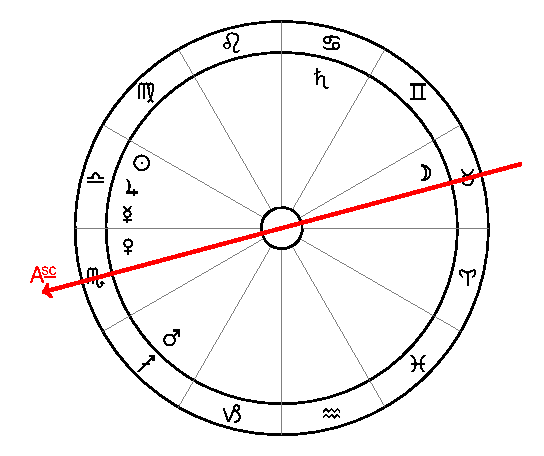
\includegraphics[width=.68\textwidth]{charts/7_6_18}
\caption{Chart 95 [VII.6.18, GH L120, IX] }
\label{fig:chart95}
\end{wrapfigure} 

An example: \Sun, \Jupiter, \Mercury\, in \Libra, \Moon\, in \Taurus, \Saturn\, in \Cancer, \Mars\, in \Sagittarius,
\Venus, Ascendant in \Scorpio, klima 2\footnote{\textit{Greek Horoscopes} dates the chart to September 28, 120 CE about 8 a.m.}.

During his 40th year he was condemned to exile. The 40th year
was indicated by the superior aspect of \Saturn\, to \Libra: 32 degrees for \Cancer\footnote{The rising times of \Cancer\, in klima 2, System A for Alexandria are 31°53'20''.}, plus 8 for \Libra\, <=\Venus> \textbf{/278P/} total 40. Also the opposition of the \Moon\, to \Venus\, <was operative>: 25 for \Taurus\, <=\Moon>\footnote{The 25 probably came from \Taurus's rising time of 24°20'00'' in klima 2, System A for Alexandria rather than from the \Moon.} plus 15 for \Scorpio\, <=\Mars> total 40. Consequently the results were activated through female persons and
for the purpose of profit. And again the “contact” of the \Moon\, with \Mars\, <was operative>: 25 for the \Moon\, plus 15 for \Mars\, total 40.

(As \mndl the King says: “Let the \Moon\, be in any sign or at an angle, and let the star of \Mars\, be just preceding or just following the \Moon\, in the contiguous sign; then the \Moon\, has ‘contact’ with it. And so, even if the star is not in the same sign as the \Moon, but is found in the adjoining sign, or in the sign in square or in opposition, then consider the contact to be solid. Sum up their periods or the rising times of the signs to forecast the chronocratorship”.)

First of \mnm all, as we have said before, it is necessary to begin with the overall forecast, then to investigate how the stars are configured, whether these configurations are benefic or bad, in what place they occur, and what this can signify; then investigate the phases of the stars in conjunction or in aspect. Having done this, predict the effects at the allotments. For \mndl instance, the aspect of opposition or of square is not always malefic, but is occasionally <benefic>. Just as <this aspect’s> influence is changed in the overall forecast by its place, its aspect, its angle, or the nature of another star, in the same way, its influence in the distribution of chronocrators is changed or is strengthened by the current transits of the stars. It is necessary to pay attention to the transits of the stars, so that these directions may prove to be accurate and to have an easily recognizable force.

\textbf{/291K/} In order not to seem to be elaborating the same rules over and over, I will append what the King has said about these matters, in his own words.
\begin{quote}
“Every star, whether situated in its proper place or square to its place, if it is beneficial or harmful to the nativity…at a similar place it is damaging to the chronocratorships of the nativity. If one is helpful, the other harmful, and both are at their proper places or square with those places, the star which brings gain will make the distribution when it comes to the place of the malefic; the other star will take away what it previously distributed, because when either is situated in square, the one becomes the bestower, the others (since it is in aspect with the giver) exhibits a lessening of the damage.”
\end{quote}

Again the King says:
\begin{quote}
“It is necessary to consider how the star which rules the chronocratorship is located relative to the \textbf{/279P/} character of the nativity, and <it is also necessary> to consider the places of control, accomplishment, and harm. The <places> where the stars happen to be located must be considered not only at the beginning of the chronocratorship, but also in the succeeding period, and the transits of the remaining stars must be taken into account, viz. the transits which aspect or sit with the ruler of the period, with \Mercury\, and the \Moon\, factored into the interpretation. For it is possible at the beginning of the period, even though these stars are favorable, that the benefic can be at the Place of Accomplishment or can be making a transit <of the Place> at any given period, and that a malefic
can also be in transit. If so, even though the chronocratorship is good, a loss of revenue will occur. Vice-versa, even though the chronocratorship if reversed <=negative>, if a benefic is in the Place of Accomplishment, and if the malefic is operative with respect to the nativity, for as long as the malefic is chronocrator, during that time the period will be full of accomplishment, with the chronocratorship adverse to nothing. The <malefic> however will show itself by the difficulties and repulsions inherent in it. In either case observe the transits of each star \textbf{/292K/} into the sign which most concerns the nativity.

“Carefully examine the motion of the \Moon, because whenever it is rising, beheld by \Mars\, or \Saturn\, square to the right of left, one must beware of the transmission—which will be in no way beneficial. If this happens in the chronocratorship of a malefic, e.g. in the chronocratorship of the star of \Mars, the native will come into close confinement or be involved with wounds. 

If the star of \Mercury\, is associated in this chronocratorship, i.e. by being in conjunction with the star of \Mars\, or by being in one of the signs belonging to the star of \Mars, it indicates that the assault or imprisonment will occur because of documents. \Saturn\, in aspect or in conjunction <shows it occurs> because of old matters, ancestral matters or the like, or because of an older person. 

If the star of \Venus\, is chronocrator, and if the star of \Mars\, happens to be in the houses of the star of \Venus, <the attack occurs> because of a female person. 

If the star of \Jupiter\, is chronocrator and if the star of \Mars\, is in the houses of \Jupiter, <it occurs> because of royalty or magnates.

“The native obtains great advancement if the star of \Jupiter, while being chronocrator, is at MC or in the Place of Accomplishment with the star of \Mars. When \Jupiter\, and \Mars\, are providing the
active impulse, it will be necessary to see if the star of \Saturn\, is coming into a transit or \textbf{/280P/} opposition, with the result that the chronocratorship of occupations becomes contrary. 

If the star of \Mercury\, is the ruler, and if the star of \Jupiter\, receives the chronocratorship from \Mercury, the native will advance in business and will fare well at those times. 

If <\Mercury> is favorably situated at the nativity, the native will engage in greater activities, proportionate to the distinction of the nativity—for this is changed to that and that is changed to this by differences in the hours of birth.

“If the places appropriate to the nativity seem invalid, judging from the positions of the stars, and if the chronocrator bestows anything (as we previously said, this is the star which is at the Place of Accomplishment), despite being profitable, it causes the income to be transitory because of the inappropriate asterisms at the nativity. The things which are granted by the asterisms proper to a nativity remain valid if they are appropriately given at a chronocratorship, i.e. if most of the benefic stars are associated with either one, are in the signs which pertain to the nativity, and are in aspect with the star which rules the chronocratorship at the time of the nativity.

“The star \textbf{/293K/} of \Saturn\, coming into the place brings reversals and the chilling of affairs; if it comes into a place of <several> stars in conjunction and if the star of \Mars\, has the Place of Accomplishment while the star of \Saturn\, has the Place of Employments, it brings mortal danger. 

In every case the star of \Saturn\, in the Sign of Accomplishment must be considered harmful. <It is also harmful> when in opposition to this Place and to the places of the stars of \Mars, \Venus, and \Mercury, depending on its relationship to any of them. The same is true of the star of \Mercury\, when it is in the places of the \Moon\, and in its own signs, while aspected by \Mars\, and \Saturn. Likewise for the star of \Venus. 

Every star when suitably located in its signs at the nativity … in the places of the \Sun\, and \Moon, and interwoven in the previously mentioned combined relationships. They reveal a similar type of result when the ruler of the chronocrator shares control with the remaining
stars which are associated with it.

“In every case the phases of the \Moon\, waxing from new to the quarter must be observed, particularly in the X Sign <=MC> (as was mentioned) and when aspected by malefics. If the stars of
\Mars\, and \Saturn\, behold the opposing place at the time of the nativity, with the \Moon\, passing through the ruling places … The \Moon\, is helpful \textbf{/281P/} when it is in the place of benefics, if indeed it is discovered to be in the places which are opportune for the nativity.”
\end{quote}

O Marcus, I have researched and discovered these matters with much ascetic labor, and I have compiled and published these systems. Consequently, I adjure you by the \Sun, the \Moon, and the orbits of the five stars, by Nature, Providence, and the four elements, not to share this too quickly with any unlearned person nor with any chance acquaintance, but to consider my labor, my longing, and my long devotion to and research of these matters. 

Estimating this work of years to be worth much money, I have left it to you, for money is easily spent and attracts envy and treachery, but my compositions will bring you a livelihood, fame, honor, pleasure, and profit, if you handle them in an orderly, secure manner (as I have described above), not in a controversial or trivial manner. And considering the exertion to be the same as if you yourself had compiled this—but indeed \textbf{/294K/} you did exert yourself when you received this art and when you were selected, giving a worthy recompense. Share this knowledge with those who are capable of it. In so doing, you will glorify both me and my science, and you will benefit yourself and show yourself to be diligent and a lover of beauty.
May your wishes be fulfilled if you keep your oath. I have finished.

The End of Book VII of the Genethliology to Daphne of Vettius Valens.

\newpage